\documentclass[a4paper,14pt]{extarticle}
\usepackage{fontspec}
\setmainfont{Times New Roman}
\usepackage[ukrainian]{babel}
\usepackage{amsmath, amssymb}
\usepackage{graphicx}
\usepackage{geometry}
\usepackage{float}
\usepackage{indentfirst}
\usepackage{booktabs}
\usepackage{caption}

\geometry{left=25mm, right=15mm, top=20mm, bottom=20mm}
\linespread{1.25}

\begin{document}
	
	\begin{titlepage}
		\begin{center}
			МІНІСТЕРСТВО ОСВІТИ І НАУКИ УКРАЇНИ\\
			ОДЕСЬКИЙ НАЦІОНАЛЬНИЙ УНІВЕРСИТЕТ ІМЕНІ І. І. МЕЧНИКОВА\\
			Факультет математики, фізики та інформаційних технологій\\
			Кафедра оптимального керування і економічної кібернетики\\[2cm]
			
			\textbf{\Large ЗВІТ}\\
			\textbf{з лабораторної роботи № 5}\\
			з дисципліни «Системи комп’ютерного зору»\\
			\textbf{Тема: «Стереобачення, побудова карт диспаратності та 3D-реконструкція»}\\[2cm]
			
			\begin{flushright}
				\textbf{Виконила:}\\
				студентка 3 курсу\\
				спеціальності «Прикладна математика»\\
				Овчарук Єлизавета Євгеніївна\\[1cm]
				
				\textbf{Перевірив:}\\
				доцент, к. ф.-м. н.\\
				Мороз Володимир Володимирович
			\end{flushright}
			
			\vfill
			Одеса — 2026
		\end{center}
	\end{titlepage}
	
	\newpage
	\tableofcontents
	\newpage
	
	\section*{Вступ і мета роботи}
	\addcontentsline{toc}{section}{Вступ і мета роботи}
	\textbf{Мета роботи:} Дослідити принципи роботи стереобачення, реалізувати алгоритми локального (Block Matching) та напівглобального (SGBM) пошуку відповідностей для побудови карт диспаратності. Здійснити перехід від піксельних зсувів до фізичної глибини, виконати кількісну оцінку за еталоном (Ground Truth) та побудувати 3D-модель (хмару точок) сцени.
	
	\textbf{Завдання:}
	\begin{enumerate}
		\item Завантажити стереопару та ідеальні дані (Ground Truth) з датасету Middlebury.
		\item Обчислити карти диспаратності за допомогою алгоритмів StereoBM та StereoSGBM.
		\item Провести сітку експериментів, дослідивши вплив параметрів \texttt{numDisparities}, \texttt{blockSize} та \texttt{uniquenessRatio} на якість та час роботи.
		\item Розрахувати карту глибини у міліметрах, використовуючи калібрувальні дані камери.
		\item Провести кількісну оцінку якості карти диспаратності за еталоном (частка пікселів з похибкою $>1$~px).
		\item Згенерувати 3D-хмару точок, застосувавши фільтрацію недійсних пікселів та обмеження по глибині.
		\item Проаналізувати типові зони помилок алгоритмів (оклюзії, однорідні текстури, відблиски).
	\end{enumerate}
	
	\section{Теоретичні відомості}
	\subsection{Диспаратність та відновлення глибини}
	У стереобаченні для двох паралельно вирівняних (ректифікованих) камер відповідні точки на лівому та правому зображеннях лежать на одній епіполярній лінії (одному рядку). Різниця їх горизонтальних координат називається \textbf{диспаратністю} (disparity): $d = x_L - x_R$.
	
	Маючи фокусну відстань камери $f$ та базову відстань між оптичними центрами камер $B$, фізична глибина об'єкта (відстань від площини камер) $Z$ обчислюється за формулою тріангуляції:
	\begin{equation}
		Z = \frac{f \cdot B}{d}
	\end{equation}
	З формули видно, що глибина обернено пропорційна диспаратності: чим ближче об'єкт, тим більший піксельний зсув він має.
	
	\subsection{Алгоритми Block Matching (BM) та Semi-Global Block Matching (SGBM)}
	Алгоритм \textbf{BM} шукає відповідності, порівнюючи невеликі квадратні вікна (блоки) вздовж епіполярної лінії, використовуючи суму абсолютних різниць (SAD). Він дуже швидкий, але чутливий до однорідних текстур.
	
	Алгоритм \textbf{SGBM} додатково накладає глобальні обмеження гладкості. Він мінімізує енергетичний функціонал, що штрафує за зміну диспаратності між сусідніми пікселями, що дозволяє отримувати значно щільніші та точніші карти навіть на слабкотекстурованих ділянках.
	
	\section{Практичне виконання та результати експериментів}
	Для експериментів використано стереопару мотоцикла з датасету Middlebury (\texttt{im0.png}, \texttt{im1.png}) та еталонну карту \texttt{disp0.pfm}.
	
	\subsection{Частина B. Дослідження параметрів (Сітка експериментів)}
	Було реалізовано автоматичний перебір параметрів: \texttt{numDisparities} $\in \{64, 128, 192\}$, \texttt{blockSize} $\in \{5, 9, 15, 21\}$, \texttt{uniquenessRatio} $\in \{5, 10, 15\}$. У Таблиці~1 наведено вибірку характерних результатів.
	
	\begin{table}[H]
		\centering
		\caption{Порівняння ефективності BM та SGBM}
		\begin{tabular}{cccccc}
			\toprule
			Алгоритм & numDisp & blockSz & uniqRat & Час (с) & Покриття (\%) \\
			\midrule
			BM & 64 & 5 & 5 & 0.067 & 73.93 \\
			SGBM & 64 & 5 & 5 & 1.008 & 61.01 \\
			BM & 192 & 15 & 5 & 0.129 & 57.72 \\
			\textbf{SGBM} & \textbf{192} & \textbf{15} & \textbf{5} & \textbf{2.588} & \textbf{70.63} \\
			SGBM & 192 & 15 & 15 & 2.568 & 60.76 \\
			\bottomrule
		\end{tabular}
	\end{table}
	
	\textbf{Висновок за експериментом:} Алгоритм BM працює в 15--20 разів швидше, але видає «шумну» карту з дірками. Найкращий візуальний та кількісний результат показав алгоритм SGBM при \texttt{numDisparities = 192} (оскільки реальний зсув мотоцикла на передньому плані є великим) та \texttt{blockSize = 15}.
	
	\begin{figure}[H]
		\centering
		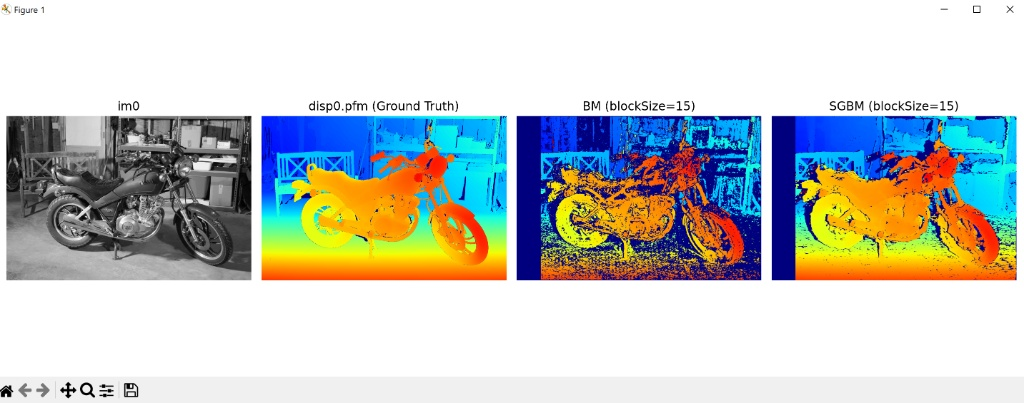
\includegraphics[width=0.85\textwidth]{map.png}
		\caption{Карта диспаратності SGBM. Ближні об'єкти (мотоцикл) мають теплі кольори (великий зсув), віддалені — холодні.}
	\end{figure}
	
	\subsection{Частина D. Оцінка за еталоном та перехід до глибини}
	Використовуючи параметри з калібрувального файлу ($f = 3997.684$, $B = 193.001$), піксельну диспаратність було конвертовано в реальну відстань (міліметри).
	
	\begin{figure}[H]
		\centering
		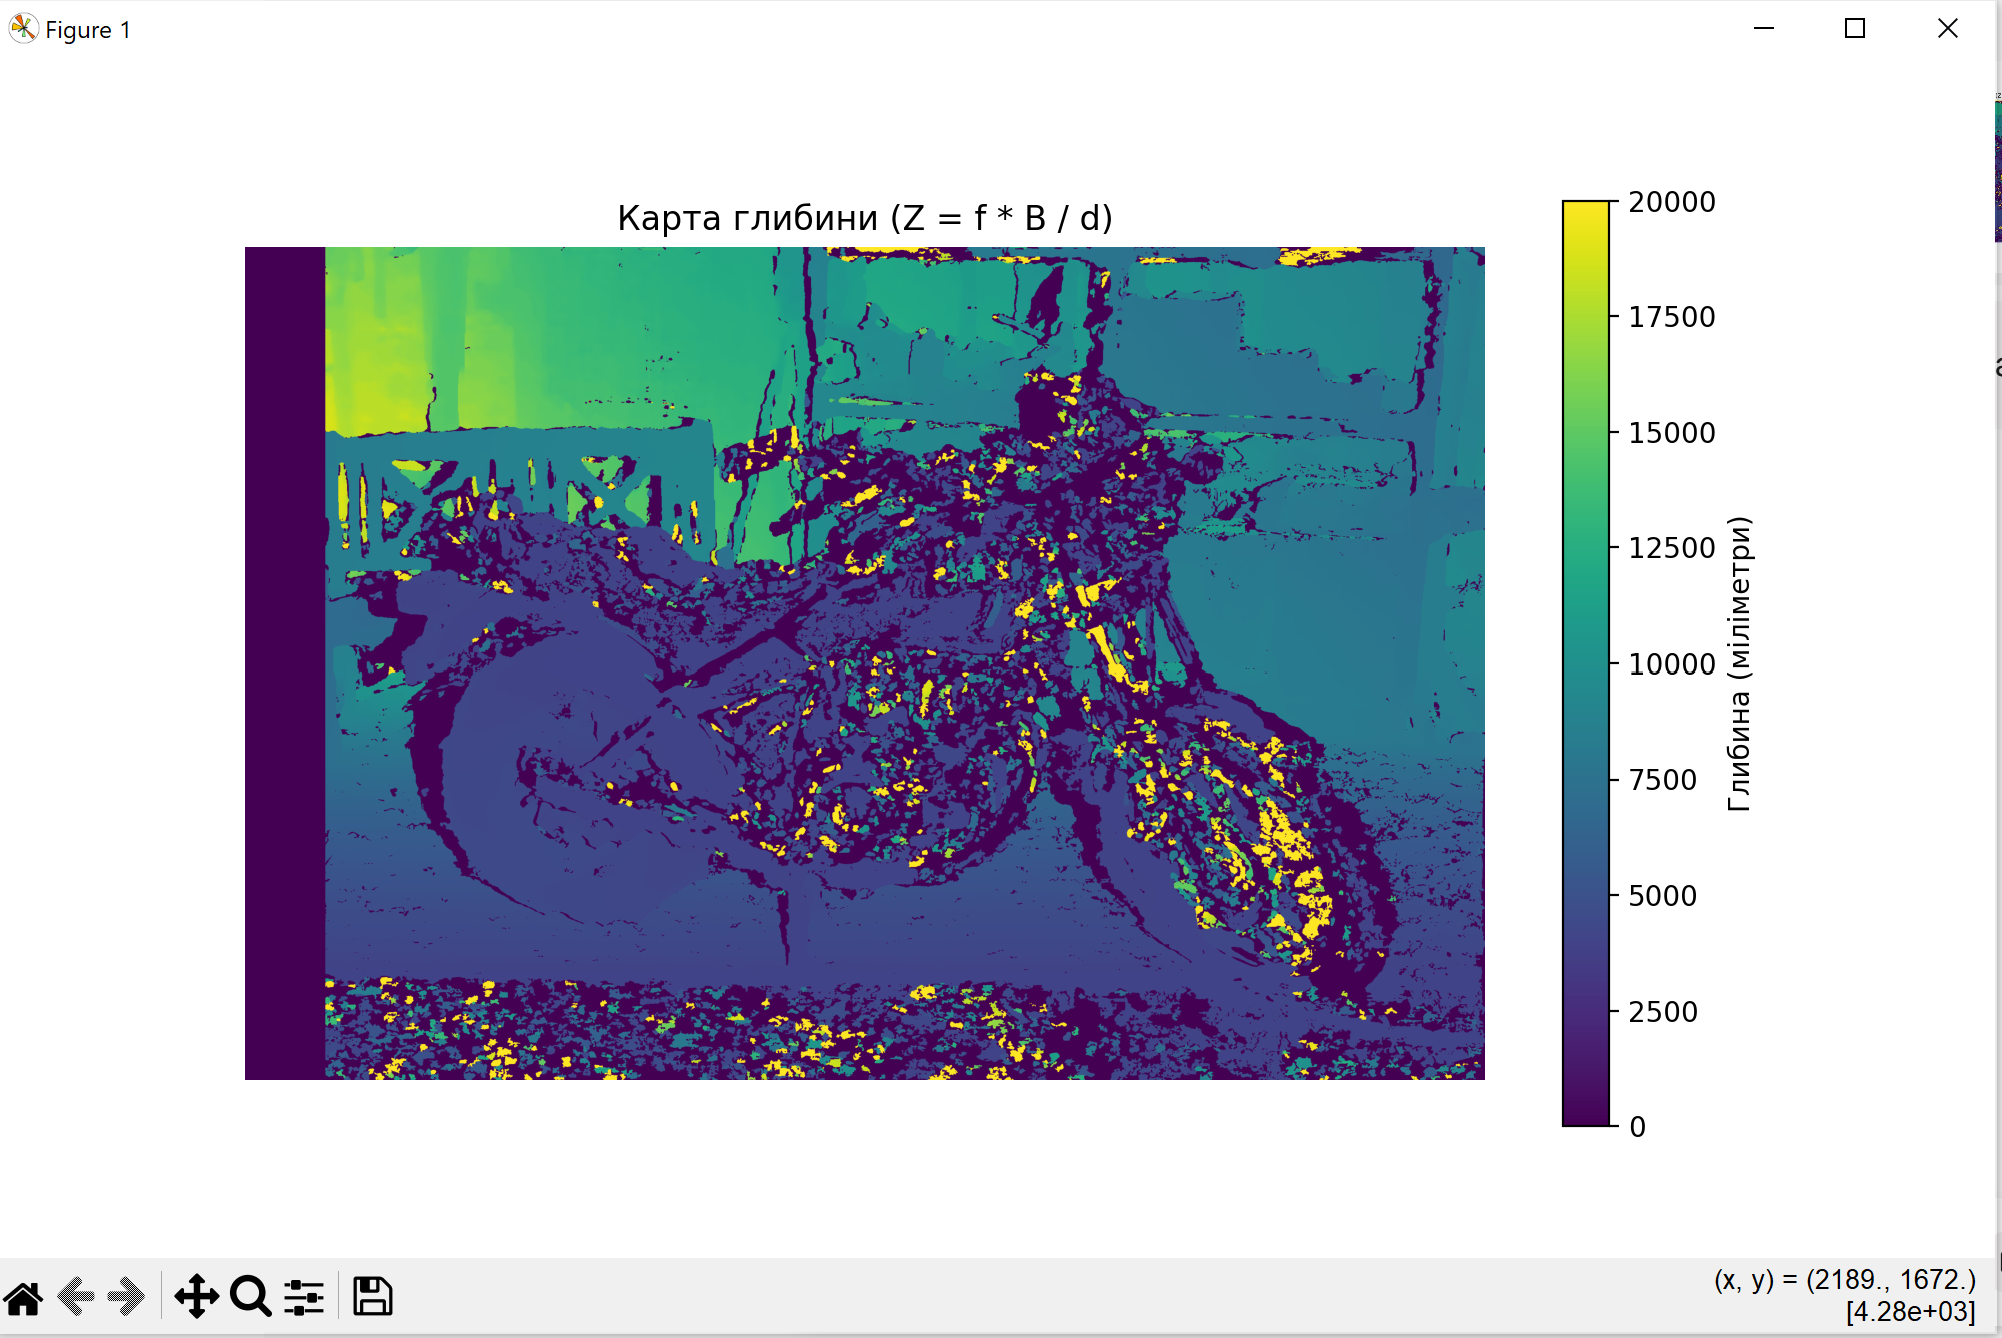
\includegraphics[width=0.85\textwidth]{depth.png}
		\caption{Карта глибини ($Z$). Мотоцикл знаходиться на відстані $\approx 3$--$5$ метрів (темно-синій колір), фон $\approx 10$--$15$ метрів (зелено-жовтий колір).}
	\end{figure}
	
	Кількісна оцінка якості найкращої карти SGBM за еталоном (Ground Truth):
	\begin{itemize}
		\item Загальне покриття нашої карти: \textbf{70.21\%}
		\item Частка пікселів з похибкою $>1$ піксель: \textbf{43.92\%}
	\end{itemize}
	Це означає, що понад 56\% розпізнаних алгоритмом пікселів мають ідеальну точність з відхиленням менше 1 пікселя від еталону.
	
	\subsection{Крок 12. Побудова хмари точок (3D-реконструкція)}
	Для генерації 3D-моделі було застосовано матрицю перетворення $Q$ та функцію \texttt{cv2.reprojectImageTo3D}. 
	Для покращення якості моделі виконано фільтрацію: відкинуто недійсні пікселі ($Z \le 0$), застосовано медіанний фільтр для видалення шуму, а також обмежено діапазон глибини (відкинуто фон, що знаходиться далі ніж 6.5 метрів). Результат візуалізовано у просторі $\mathbb{R}^3$.
	
	\begin{figure}[H]
		\centering
		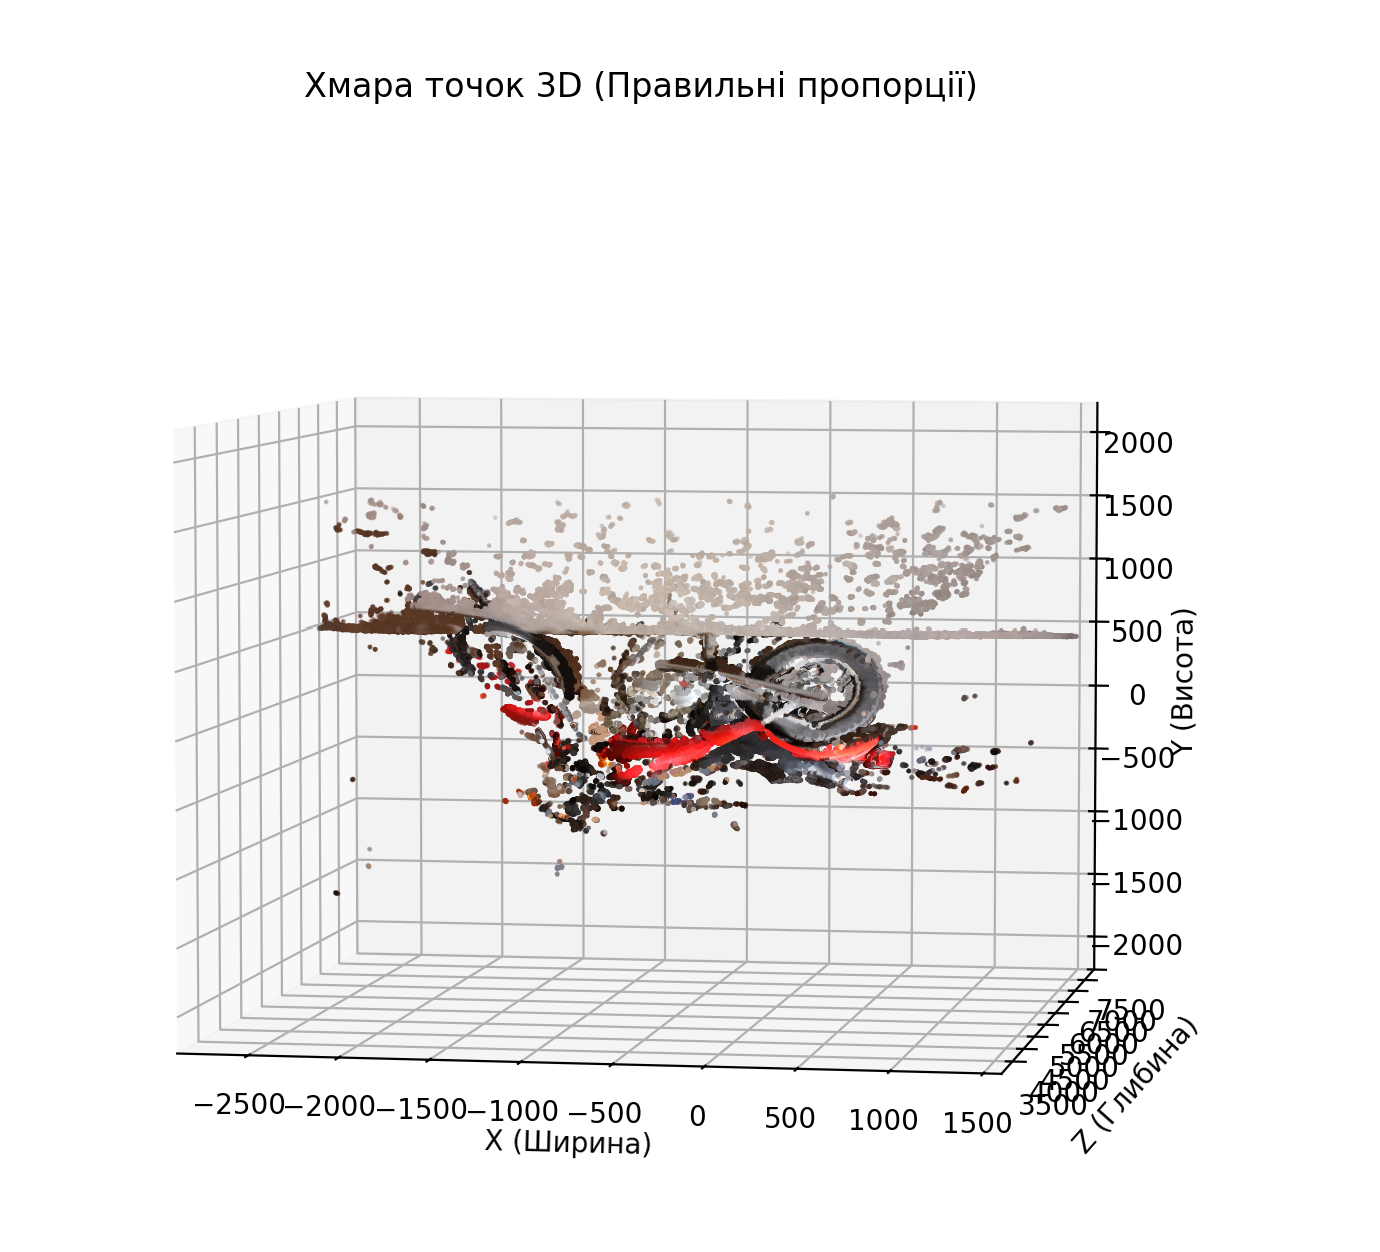
\includegraphics[width=0.85\textwidth]{cloud.png}
		\caption{3D-реконструкція об'єкта переднього плану (хмара точок).}
	\end{figure}
	
	\subsection{Частина E. Аналіз помилок (Крок 14)}
	Під час аналізу побудованих карт диспаратності було виявлено типові для стереобачення проблеми:
	\begin{enumerate}
		\item \textbf{Зона оклюзії (темна смуга зліва кадру):} Оскільки камери рознесені на базу $B$, ліва камера не бачитиме частину простору біля лівого краю через обмеження кута огляду та перекриття. Для цих пікселів фізично не існує відповідника на правому кадрі.
		\item \textbf{Однорідні поверхні (підлога):} На бетоні без чіткої текстури квадратичні блоки виглядають однаково. Алгоритм не може знайти унікальний мінімум функції вартості, що призводить до появи «дірок» (особливо в алгоритмі BM).
		\item \textbf{Відблиски металу:} Яскраві відблиски на баку мотоцикла порушують базове припущення стереозору про сталість яскравості (Lambertian assumption), оскільки відблиск зміщується залежно від ракурсу камери.
	\end{enumerate}
	
	\section*{Висновки}
	\addcontentsline{toc}{section}{Висновки}
	\begin{enumerate}
		\item Досліджено принципи роботи стереобачення та виконано реконструкцію глибини сцени. Продемонстровано, що значення глибини обернено пропорційне піксельній диспаратності.
		\item У результаті порівняння алгоритмів встановлено, що SGBM значно перевершує локальний BM за якістю та щільністю покриття, нівелюючи проблеми однорідних ділянок завдяки глобальній оптимізації, проте вимагає значно більше часу на обчислення.
		\item Шляхом перебору параметрів знайдено оптимальну конфігурацію (\texttt{numDisparities=192, blockSize=15}), яка дозволила досягти субпіксельної точності (похибка $<1$~px) для понад 56\% розпізнаних точок порівняно з ідеальним Ground Truth.
		\item Успішно здійснено перехід від двовимірної карти зсувів до реальних фізичних координат у міліметрах та побудовано відфільтровану 3D-хмару точок об'єкта переднього плану.
		\item Проаналізовано фундаментальні обмеження класичного стереобачення, пов'язані з оклюзіями, відсутністю текстур та дзеркальними відблисками.
	\end{enumerate}
	
\end{document}